\documentclass[fleqn,a4paper,11pt]{article}
\usepackage{etex}
\usepackage[utf8]{inputenc}
\usepackage[T1]{fontenc}
\usepackage[english]{babel}
\usepackage{makecell}
\input{_Preambules}
%\usepackage{boiboites}
%\input{../../PreambuleTD}
\usepackage{enumitem}
\newcounter{num}
\newcommand{\ex}{\addtocounter{num}{1}
\textbf{Exercice \no\thenum.}}
\usepackage{listings}
\input{Preambulepython}

%\setboolean{eleve}{false} %doc de l'élève
%\setboolean{Profsanssol}{false}
\setboolean{prof}{true}
\geometry{hmargin=2.5cm,vmargin=2.5cm}

\EnteteDevoir{ESM/SLA Robotic}{EF 15/02/2024}{Neural Network}


\title{}
\author{}




\begin{document}

	\Titre{Evaluation }
%		 \Titre{Exercices à préparer}

%	\begin{center}
%		
%		\fbox{	\begin{minipage}[h]{15cm} 
%				\begin{center}	 {\small Le devoir comporte 5 exercices et dure 01h50. 
%						
%						La calculatrice et les documents {sont autorisés}.
%						
%						%Les exercices ...  est à rendre sur une \textbf{copie séparée}.
%						%Le sujet comporte 4 pages et 4 exercices indépendants.
%						
%						%Barème indicatif : Ex1 (5 pts), Ex2 (5 pts), Ex3 (5 pts), Ex4 (5 pts)
%					}
%				\end{center}
%			\end{minipage}
%		}
%		
%	\end{center}
	\vspace{1cm}
	
\paragraph{Exercise 1: }

Let $ReLu$ be the Relu function: 

\begin{python}
def Relu(y):
  if y<0:
	return 0
  else:
	return y
\end{python}

We consider this neuron with 2 inputs and a bias:
\begin{center}
\begin{tikzpicture}[scale=0.5]
\draw[thick,fill=black!10] (0,0) circle (3);
\node at (150:9) {$x_1$};
\node at (190:9) {$x_2$};
\draw[ultra thick]  (150:3) -- (150:8)node[pos=0.3,above]{$3$};;
\draw[ultra thick]  (190:3) -- (190:8) node[pos=0.3,above]{$-2$};
\draw[-o,ultra thick]  (210:3) -- (210:8) node[pos=0.3,above]{$-1$};
\draw[->,>=latex,ultra thick] (0:3) --  (8,0) node[right] {};
\node[below right] at (-15:3) {$ReLu$};
\end{tikzpicture}  
\end{center}
Compute the output when the input is $(x_1,x_2) = (1,-3)$ and then if the input is $(x_1,x_2) = (3,1)$. 


%\rep{We compute $-3 \times 1 + 2 \times (-3) -1 <0$ so the output is $0$.  }

\vspace{2em} %\hfill \newpage
\paragraph{Exercise 2: } Design a neuron that realizes the classification between blue circles and red squares as following. Explain your choices.

\begin{center}
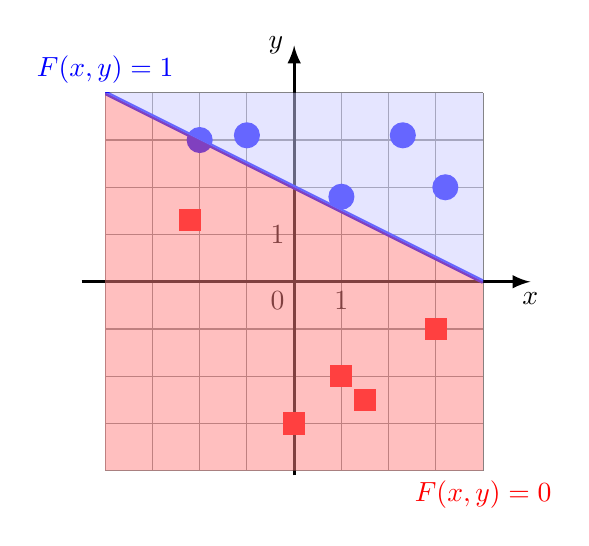
\begin{tikzpicture}[scale=0.6]
\tikzstyle{rouge} = [fill,rectangle,red,scale=1.2];
\tikzstyle{bleu} = [fill,circle,blue] ;

\draw[gray] (-4,-4) grid ++(8,8);
\draw[->,>=latex, very thick,black] (-4.5,0)--(5,0) node[below] {$x$};
\draw[->,>=latex, very thick, black] (0,-4.1)--(0,5) node[left] {$y$};

\node[below left] at (0,0) {$0$};
\node[left] at (0,1) {$1$};
\node[below] at (1,0) {$1$};

\foreach \x/\y in {-2/3,3.2/2,-1/3.1,1/1.8,2.3/3.1}{
	\node[bleu] at (\x,\y) {};
}
\foreach \x/\y in {1/-2,3/-1,1.5/-2.5,0/-3,-2.2/1.3}{
	\node[rouge] at (\x,\y) {};
}

\begin{scope}[even odd rule]
\clip (-4,-4) rectangle (4,4);
\draw[blue,ultra thick] (-4,4) -- (4,0);
\fill[red!50,opacity=0.5] (-4,4) -- (-4,-4) --(4,-4)--(4,0) -- cycle;
\fill[blue!20,opacity=0.5] (-4,4) -- (-4,4) --(4,4)--(4,0) -- cycle;

\end{scope}

\node[scale=1,red,below] at (4,-4) {$F(x,y)=0$};
\node[scale=1,blue,above] at (-4,4) {$F(x,y)=1$};
%\node[red,below] at (-1,-4) {$y=8x+4$};

\end{tikzpicture}
\end{center}

%\rep{ We want to separate the plane into to half planes. One can consider the red line defined by $y=5x/8+1/2$ that is $5x-8y+4 = 0$ or another line which separates as well, for example $5x-8y=0$.  So this neuron can fit to this problem.
%
%\begin{center}
%	\begin{tikzpicture}[scale=0.5]
%	\draw[thick,fill=black!10] (0,0) circle (2);
%	\node at (150:9) {$x$};
%	\node at (190:9) {$y$};
%	\draw[ultra thick]  (150:3) -- (150:8)node[pos=0.3,above]{$5$};;
%	\draw[ultra thick]  (190:3) -- (190:8) node[pos=0.3,above]{$-8$};
%	\draw[-o,ultra thick]  (210:3) -- (210:8) node[pos=0.3,above]{$4$};
%	\draw[->,>=latex,ultra thick] (0:3) --  (8,0) node[right] {};
%	\node[below right] at (-15:3) {$H$};
%	\end{tikzpicture}  
%\end{center}
%
%  } 

%\newpage \hfill \newpage
\pagebreak
\paragraph{Exercise 3: }

Explain with a  graphic what this neural network can realizes:

\begin{center}
	\begin{tikzpicture}[scale=1.5]
\def\layersep{2cm}
\tikzstyle{every pin edge}=[thick]
\tikzstyle{neuron}=[circle,fill=black!25,minimum size=12pt,inner sep=0pt]
\tikzstyle{entree}=[];
\tikzstyle{input neuron}=[neuron, fill=green!50];
\tikzstyle{output neuron}=[neuron, fill=red!50];
\tikzstyle{hidden neuron}=[neuron, fill=blue!50];
\tikzstyle{annot} = [text width=4em, text centered]

% Entree
\node[entree,blue] (E-1) at (-\layersep,-0.5) {$x$};
\node[entree,blue] (E-2) at (-\layersep,-2.5) {$y$};

% Premiere couche
\node[input neuron] (I-1) at (0,0) {};
%\node[input neuron] (I-2) at (0,-1.5) {};
\node[input neuron] (I-3) at (0,-3) {};

\node[above right=0.8ex,scale=0.7] at (I-1) {$H$};
%\node[above right=0.8ex,scale=0.7] at (I-2) {$H$};
\node[below right=0.8ex,scale=0.7] at (I-3) {$H$};

\node[below right=0.8ex,scale=0.7] at (I-1) {};
\node[below right=0.8ex,scale=0.7] at (I-3) {};
%\node[below right=0.8ex,scale=0.7] at (I-2) {};

% \node[above right=0.8ex,blue] at (I-1) {$s_1$};
% \node[above right=0.8ex,blue] at (I-2) {$s_2$};
% \node[above right=0.8ex,blue] at (I-3) {$s_3$};

%Seconde couche et sortie
\node[output neuron] (O) at (\layersep,-1.5 cm) {};
\node[below right=0.8ex,scale=0.7] at (O) {};
\node[above right=0.8ex,scale=0.7] at (O) {$H$};

% Arrete et poids
\path[thick] (E-1) edge node[pos=0.8,above,scale=0.7]{$-1$} (I-1) ;
\path[thick] (E-2) edge node[pos=0.8,above left,scale=0.7]{$1$} (I-1);
\draw[-o,thick] (I-1) to node[midway,below right,scale=0.7]{$-1$} ++ (-110:0.8);

%\path[thick] (E-1) edge node[pos=0.8,above,scale=0.7]{$1$} (I-2);
%\path[thick] (E-2) edge node[pos=0.8,above,scale=0.7]{$1$} (I-2);
%\draw[-o,thick] (I-2) to node[midway,below right,scale=0.7]{$-2$} ++ (-130:0.8);

\path[thick] (E-1) edge node[pos=0.9,above right,scale=0.7]{$1$} (I-3);
\path[thick] (E-2) edge node[pos=0.8,above,scale=0.7]{$0$} (I-3);
\draw[-o,thick] (I-3) to node[midway,below right,scale=0.7]{$1$} ++ (-130:0.8);

\path[thick] (I-1) edge node[pos=0.8,above,scale=0.7]{$1$} (O);
%\path[thick] (I-2) edge node[pos=0.8,below,scale=0.7]{$1$}(O);
\path[thick] (I-3) edge node[pos=0.8,below,scale=0.7]{$1$}(O);
\draw[-o,thick] (O) to node[midway,below right,scale=0.7]{$-2$} ++ (-110:0.8) ;

% Sortie
\draw[->,thick] (O)-- ++(1,0) node[right,blue]{$F(x,y)$};

\end{tikzpicture}  
\end{center}

%\rep{This neural network has three neurons in the first layer, each one car separate the plane into to half planes. The second layer is made by only one neuron which is the AND neuron. 
%	
%	So this neural network has output $1$ if $(x,y)$ is at the intersection of the 3 half planes, $0$ if not. Precisely, can separate the plane into two parts as following:
%	
%\begin{tikzpicture}[scale=1]
%
%
%\begin{scope}[even odd rule]
%\clip (-2,-1) rectangle (8,5);
%% \draw[ blue,ultra thick] (6,2) -- (-6,-2);
%% \fill[blue!20,opacity=0.5] (6,2) -- (6,6) --(-6,6) --(-6,-2)-- cycle;
%% 
%% \draw[ green!70!black,ultra thick] (-3,6) -- (3,-6);
%% \fill[ green!70!black!20,opacity=0.5] (-3,6) -- (6,6) --(6,-6) --(3,-6)-- cycle;
%
%
%\draw[ultra thick,dashed] (1.33,0.66) -- (-10,-5);
%\draw[red,ultra thick] (1.33,0.66) -- (6,3);
%\draw[ultra thick,dashed] (6,3) -- (10,5);
%
%\draw[ultra thick,dashed] (-1,3) -- (-7,3);
%\draw[red,ultra thick] (-1,3) -- (6,3);
%\draw[ultra thick,dashed] (6,3) -- (8,3);
%
%\draw[ultra thick,dashed] (-6,8) -- (-1,3);
%\draw[ red,ultra thick] (-1,3)--(1.33,0.66);
%\draw[ultra thick,dashed] (1.33,0.66)--(6,-4);
%
%\fill[red!50,opacity=0.5] (1.33,0.66) -- (-1,3) -- (6,3) -- cycle;
%
%\end{scope}
%
%\draw[->,>=latex, very thick,gray] (-2.5,0)--(9,0) node[below] {$x$};
%\draw[->,>=latex, very thick, gray] (0,-1.5)--(0,6) node[left] {$y$};
%\draw[gray,thin] (-2,-1) grid (8,5);
%
%\node[left] at (-2,4) {$x+y-2=0$};
%\node[left] at (-2,3) {$-y+3=0$};
%\node[right] at (8,4) {$-x+2y=0$};
%
%\node[scale=1.2,red] at (2,2.3) {$F(x,y)=1$};
%
%\node at (0,0) [below left] {$0$};
%\node at (1,0) [below right] {$1$};
%\node at (0,1) [above left] {$1$};
%
%\end{tikzpicture}
%}
%\begin{enumerate}
%	\item We consider the following neuron, where $H$ is the Heaviside function:
%	
%	
%	\begin{tikzpicture}[scale=0.5]
%	
%	\draw[thick,fill=black!10] (0,0) circle (3);
%	\draw[ultra thick]  (150:3) -- (150:8)node[pos=0.2,above]{$1$} node[left]{$x$};
%	\draw[ultra thick]  (180:3) -- (180:8)node[pos=0.2,above]{$1$} node[left]{$y$};
%	\draw[-o,ultra thick]  (210:3) -- (210:8) node[pos=0.2,below]{$-2$};
%	\draw[->,>=latex,ultra thick] (0:3) --  (8,0);
%	\node[below right] at (-15:3) {$H$};
%	
%	\end{tikzpicture}  
%	
%	Which boolean operation is realized by this neuron ?
%
% \item Deduce a neural network that realizes the classification as following:
% 
% \begin{tikzpicture}
% 
% 
% \tikzstyle{rouge} = [fill,rectangle,red,scale=1.2];
% \tikzstyle{bleu} = [fill,circle,blue] ;
% 
% \draw[gray] (-4,-4) grid ++(8,8);
% \draw[->,>=latex, very thick,black] (-4.5,0)--(5,0) node[below] {$x$};
% \draw[->,>=latex, very thick, black] (0,-4.1)--(0,5) node[left] {$y$};
% 
% \foreach \x/\y in {2/1,1/-2,-3/-3,-3.2/0.6,-1/-1}{
% 	\node[bleu] at (\x,\y) {};
% }
% \foreach \x/\y in {1/2,-1.5/3,2.2/3.1}{
% 	\node[rouge] at (\x,\y) {};
% }
% 
% \begin{scope}[even odd rule]
% \clip (-4,-4) rectangle (4,4);
% %\draw[red,ultra thick] (0,4) -- (-1,-4);
% \fill[red!50,opacity=0.5] (-4,4) -- (0,0) --(4,4) -- cycle;
% \fill[blue!20,opacity=0.5](-4,4) -- (0,0) --(4,4) -- (4,-4) -- (-4,-4) -- cycle;
% 
% \end{scope}
% 
% \node[scale=1,red,below] at (2,4) {$F(x,y)=1$};
% \node[scale=1,blue,above] at (-2,-4) {$F(x,y)=0$};
%% \node[red,below] at (-1,-4) {$8x-y+4=0$};
% 
% \end{tikzpicture}
%\end{enumerate}

\vspace{2em} %\newpage \hfill \newpage

\paragraph{Exercise 4: }
Explain what this neural network can realizes: 

\begin{center}
	\begin{tikzpicture}[scale=1.5]
\def\layersep{2cm}
\tikzstyle{every pin edge}=[thick]
\tikzstyle{neuron}=[circle,fill=black!25,minimum size=12pt,inner sep=0pt]
\tikzstyle{entree}=[];
\tikzstyle{input neuron}=[neuron, fill=green!50];
\tikzstyle{output neuron}=[neuron, fill=red!50];
\tikzstyle{hidden neuron}=[neuron, fill=blue!50];
\tikzstyle{annot} = [text width=4em, text centered]

% Entree
\node[entree,blue] (E) at (-\layersep,-2.5) {$x$};

% Premiere couche
\node[input neuron] (I-1) at (0,-1) {};
\node[input neuron] (I-2) at (0,-2) {};
\node[input neuron] (I-3) at (0,-3) {};
\node[input neuron] (I-4) at (0,-4) {};

\node[above right=0.8ex,scale=0.7] at (I-1) {$H$};
\node[above right=0.8ex,scale=0.7] at (I-2) {$H$};
\node[below right=0.8ex,scale=0.7] at (I-3) {$H$};
\node[below right=0.8ex,scale=0.7] at (I-4) {$H$};

%Seconde couche et sortie
\node[output neuron] (O) at (\layersep,-2.5 cm) {};
\node[below right=0.8ex,scale=0.7] at (O) {id};

% Arrete et poids
\path[thick] (E) edge node[pos=0.8,above,scale=0.7]{$1$} (I-1) ;
\draw[-o,thick] (I-1) to node[midway,below right,scale=0.7]{$-1$} ++ (-120:0.6);

\path[thick] (E) edge node[pos=0.8,above,scale=0.7]{$-1/3$} (I-2);
\draw[-o,thick] (I-2) to node[midway,below right,scale=0.7]{$1$} ++ (-120:0.6);

\path[thick] (E) edge node[pos=0.8,above,scale=0.7]{$-1/5$} (I-3) ;
\draw[-o,thick] (I-3) to node[midway,below right,scale=0.7]{$1$} ++ (-120:0.6);

\path[thick] (E) edge node[pos=0.8,below left,scale=0.7]{$1/4$} (I-4);
\draw[-o,thick] (I-4) to node[midway,below right,scale=0.7]{$-1$} ++ (-120:0.6);

\path[thick] (I-1) edge node[pos=0.8,above,scale=0.7]{$1$} (O);
\path[thick] (I-2) edge node[pos=0.8,above,scale=0.7]{$1$}(O);
%\draw[-o,thick] (O) to node[midway,right,scale=0.7]{$-3$} ++ (120:0.8) ;

\path[thick] (I-3) edge node[pos=0.8,above,scale=0.7]{$2$} (O);
\path[thick] (I-4) edge node[pos=0.8,above,scale=0.7]{$2$}(O);
\draw[-o,thick] (O) to node[midway,below right,scale=0.7]{$-3$} ++ (-120:0.8) ;
% Sortie
\draw[->,thick] (O)-- ++(1,0) node[right,blue]{$F(x)$};

\end{tikzpicture} 
\end{center} 

%\rep{ 
%	This neural network realizes the function $\R \to \R$ as follows:
%\begin{tikzpicture}[scale=1]
%
%\draw[->,>=latex, gray] (-0.5,0)--(6,0) node[below] {$x$};
%\draw[->,>=latex, gray] (0,-0.5)--(0,4) node[left] {$y$};
%
%\draw[ultra thick,red] (-0.5,0) -- (1,0);
%\draw[ultra thick,red] (1,1) -- (3,1);
%
%\draw[ultra thick,red] (3,0) -- (4,0);
%\draw[ultra thick,red] (4,2) -- (5,2);
%\draw[ultra thick,red] (5,0) -- (6,0) node[above]{$F(x)$};
%
%\fill[black] (0,1) circle (1pt);
%\fill[black] (1,0) circle (1pt);
%
%\node at (0,0) [below left] {$0$};
%\node at (0,1) [left] {$1$};
%\node at (1,0) [below] {$1$};
%
%\node at (1,0) [below] {$1$};
%
%\node at (3,0) [below] {$3$};
%\node at (4,0) [below] {$4$};
%\node at (5,0) [below] {$5$};
%
%\draw[dashed] (1,1)--(0,1) node[left]{$1$};
%\draw[dashed] (4,2)--(0,2) node[left]{$2$};
%
%\draw[dashed] (1,0)--(1,1);
%\draw[dashed] (3,0)--(3,1);
%\draw[dashed] (4,0)--(4,2);
%\draw[dashed] (5,0)--(5,2);
%
%\end{tikzpicture}	
%}
\vspace{2em}

\paragraph{Exercise 5:}
Design a neural network which realizes the function $\R \to \R$ as follows:

\begin{tikzpicture}[scale=1]

\draw[->,>=latex, gray] (-0.5,0)--(6,0) node[below] {$x$};
\draw[->,>=latex, gray] (0,-0.5)--(0,4) node[left] {$y$};

\draw[ultra thick,red] (-0.5,0) -- (2,0);
\draw[ultra thick,red] (2,3) -- (4,3);

%\draw[ultra thick,red] (3,0) -- (4,0);
%\draw[ultra thick,red] (4,2) -- (5,2);
\draw[ultra thick,red] (4,0) -- (6,0) node[above]{$F(x)$};

\fill[black] (0,1) circle (1pt);
\fill[black] (1,0) circle (1pt);

\node at (0,0) [below left] {$0$};
\node at (0,1) [left] {$1$};
\node at (1,0) [below] {$1$};

\node at (2,0) [below] {$2$};
%\node at (3,0) [below] {$3$};
\node at (4,0) [below] {$4$};
%\node at (5,0) [below] {$5$};

%\draw[dashed] (1,1)--(0,1) node[left]{$1$};
\draw[dashed] (2,3)--(0,3) node[left]{$3$};

%\draw[dashed] (1,0)--(1,1);
\draw[dashed] (2,0)--(2,3);
\draw[dashed] (4,0)--(4,3);
%\draw[dashed] (5,0)--(5,2);

\end{tikzpicture}	
%\newpage \hfill \newpage

\end{document}
 